\documentclass{article}
\usepackage[left=1in, right=1in, top=1in, bottom=1in]{geometry}
\usepackage{graphicx}
\usepackage{subfig}
\usepackage{amsmath}

\title{One-trait Brownian Motion calibrated validation}
\author{F\'{a}bio K. Mendes and Rong Zhang}
\date{March 2019}

\begin{document}
\maketitle

\newpage

\section{Multivariate-normal likelihood class}

Priors for simulations were $\sigma^2 \sim \text{N}(0, 2)$, and $\mu \sim \text{Exp}(5)$. Tree (50 tips) was fixed, but came from a Yule prior.

\begin{figure}[!ht]
  \begin{minipage}[c]{.4\textwidth}
    \centering
    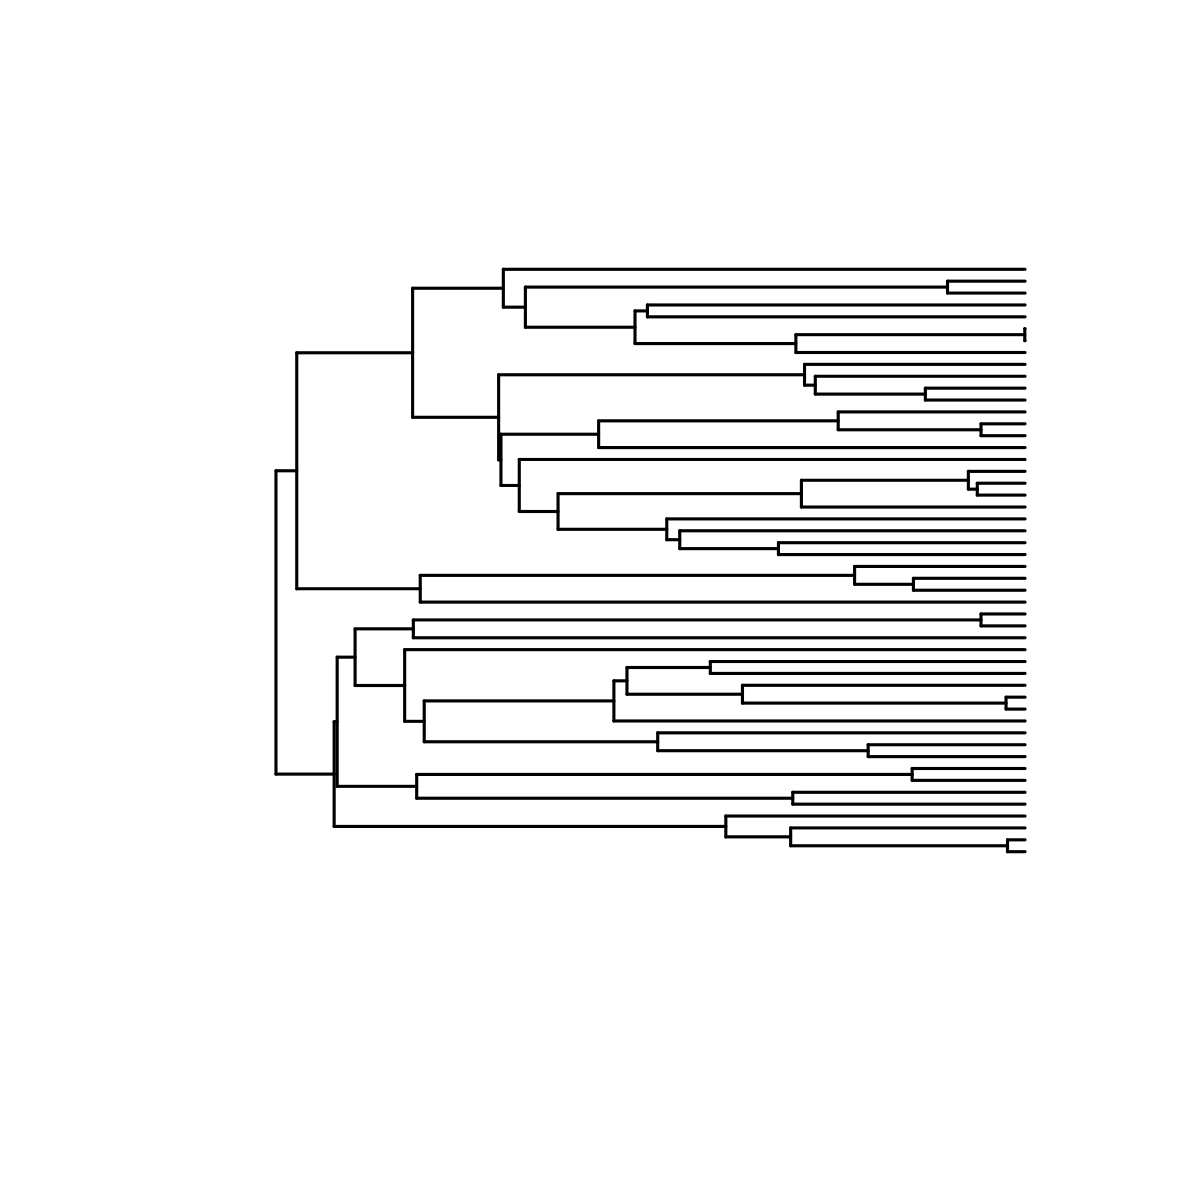
\includegraphics[width=7cm]{../BMMVN_ultra_tree.png}
  \end{minipage}
  \hfill
  \begin{minipage}{.5\textwidth}
    \centering
    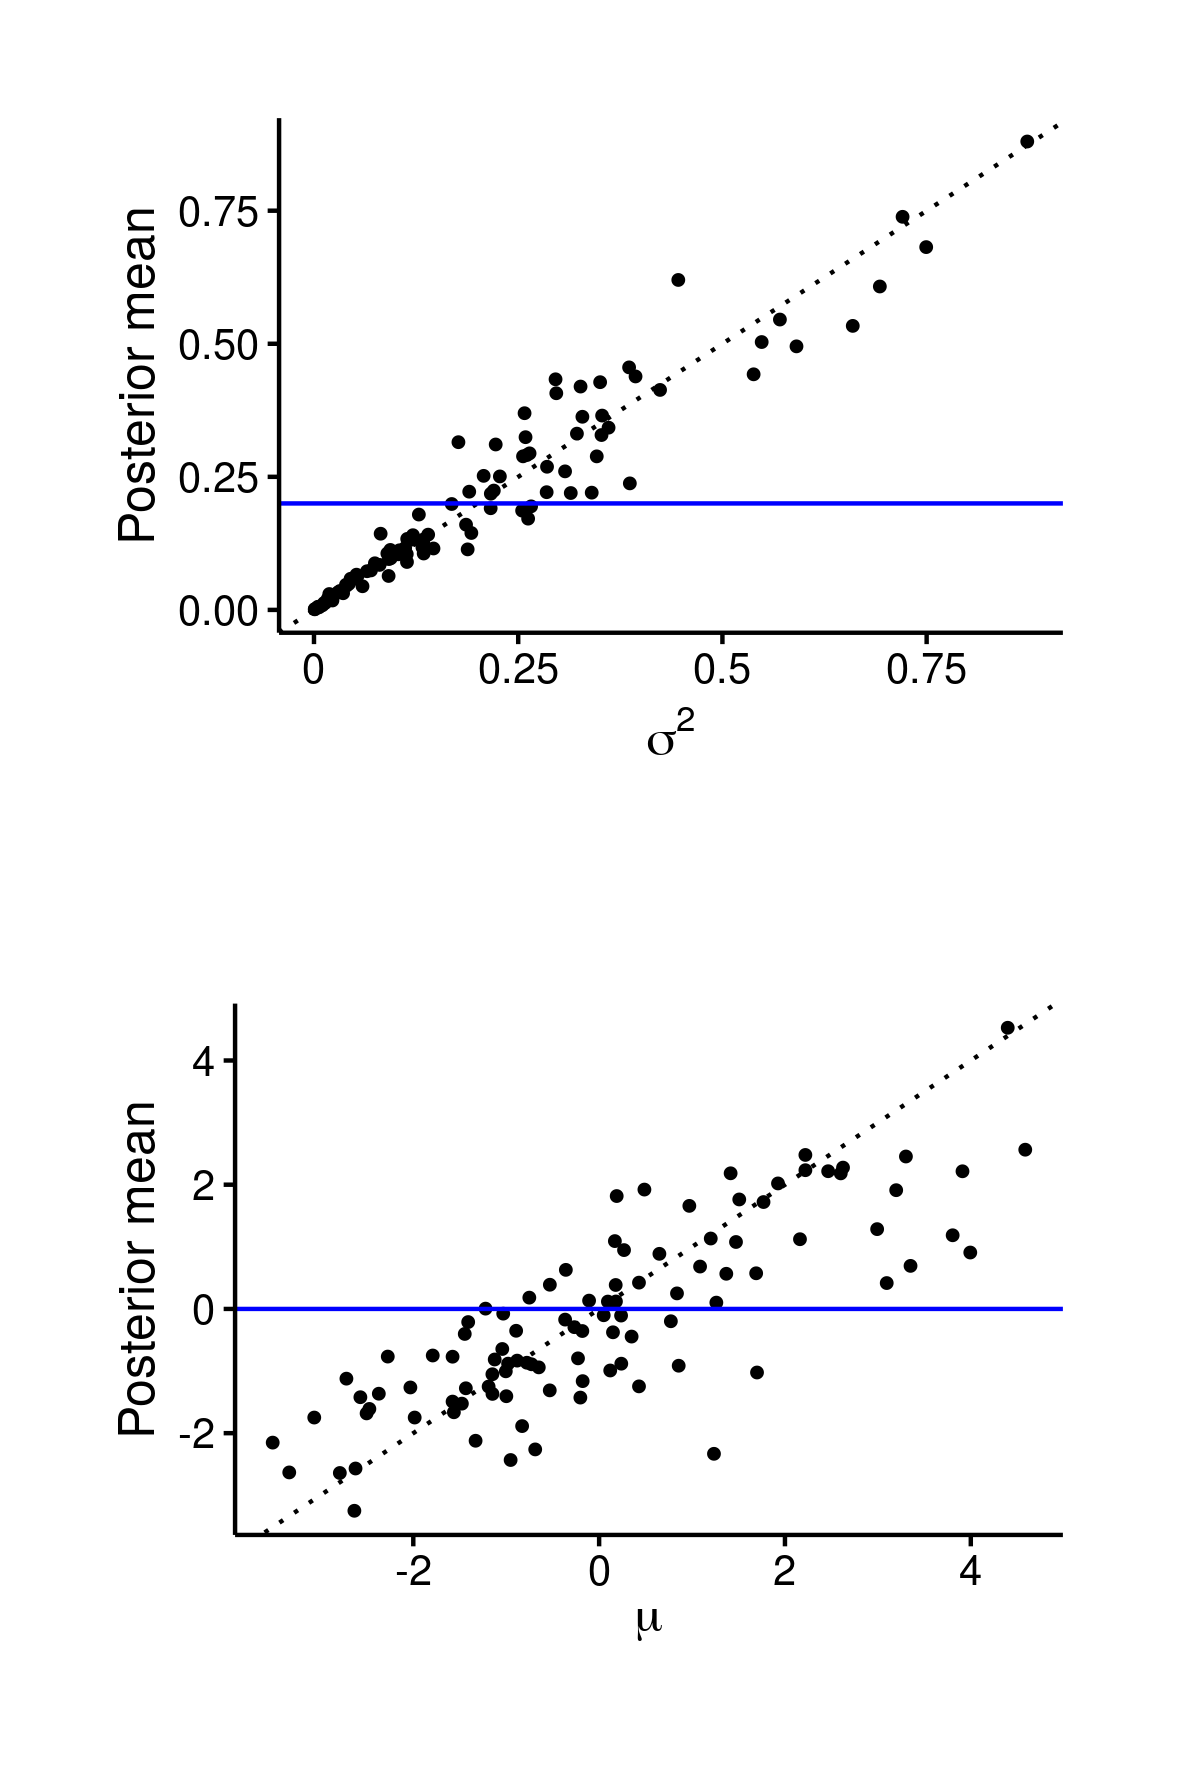
\includegraphics[width=8cm]{../BMMVN_ultra_graphs.png}
  \end{minipage}
  % \caption{The caption for both}
  % \label{mylabel:1}
\end{figure}

\begin{center}
\begin{tabular}{c | c}
    Parameter & Coverage (\%) \\\hline
    $\mu$ & 94\\
    $\sigma^2$ & 93
\end{tabular}
\end{center}

\newpage

\noindent We used the same data sets for the non-ultrametric tree. Approximately half of the tips were made short manually (0.1 length).

\begin{figure}[!ht]
  \begin{minipage}[c]{.4\textwidth}
    \centering
    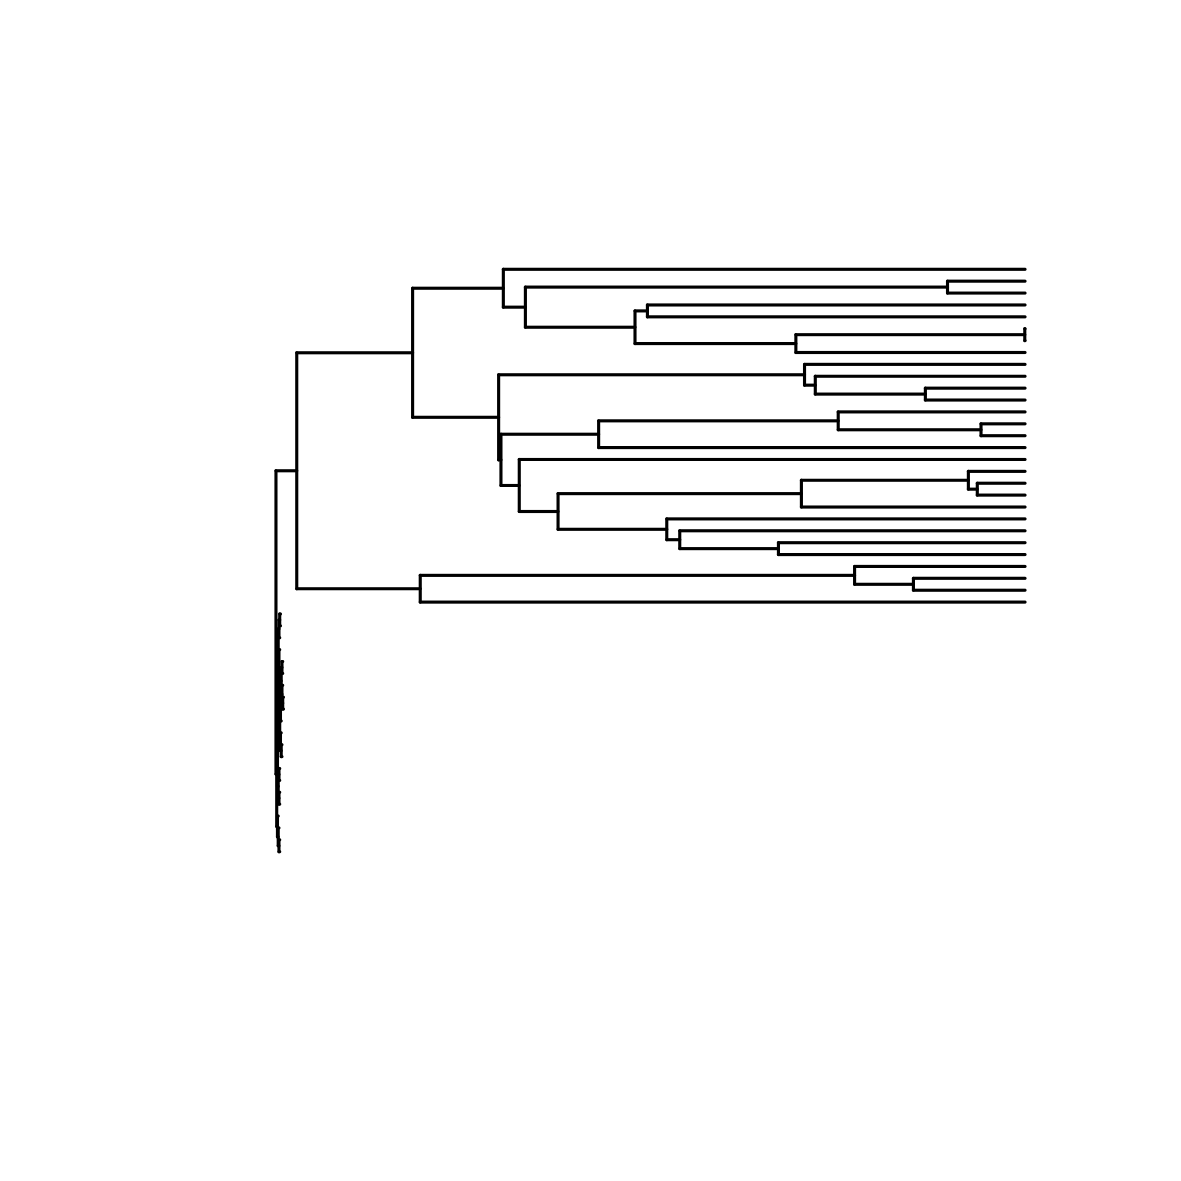
\includegraphics[width=7cm]{../BMMVN_nonultra_tree.png}
  \end{minipage}
  \hfill
  \begin{minipage}{.5\textwidth}
    \centering
    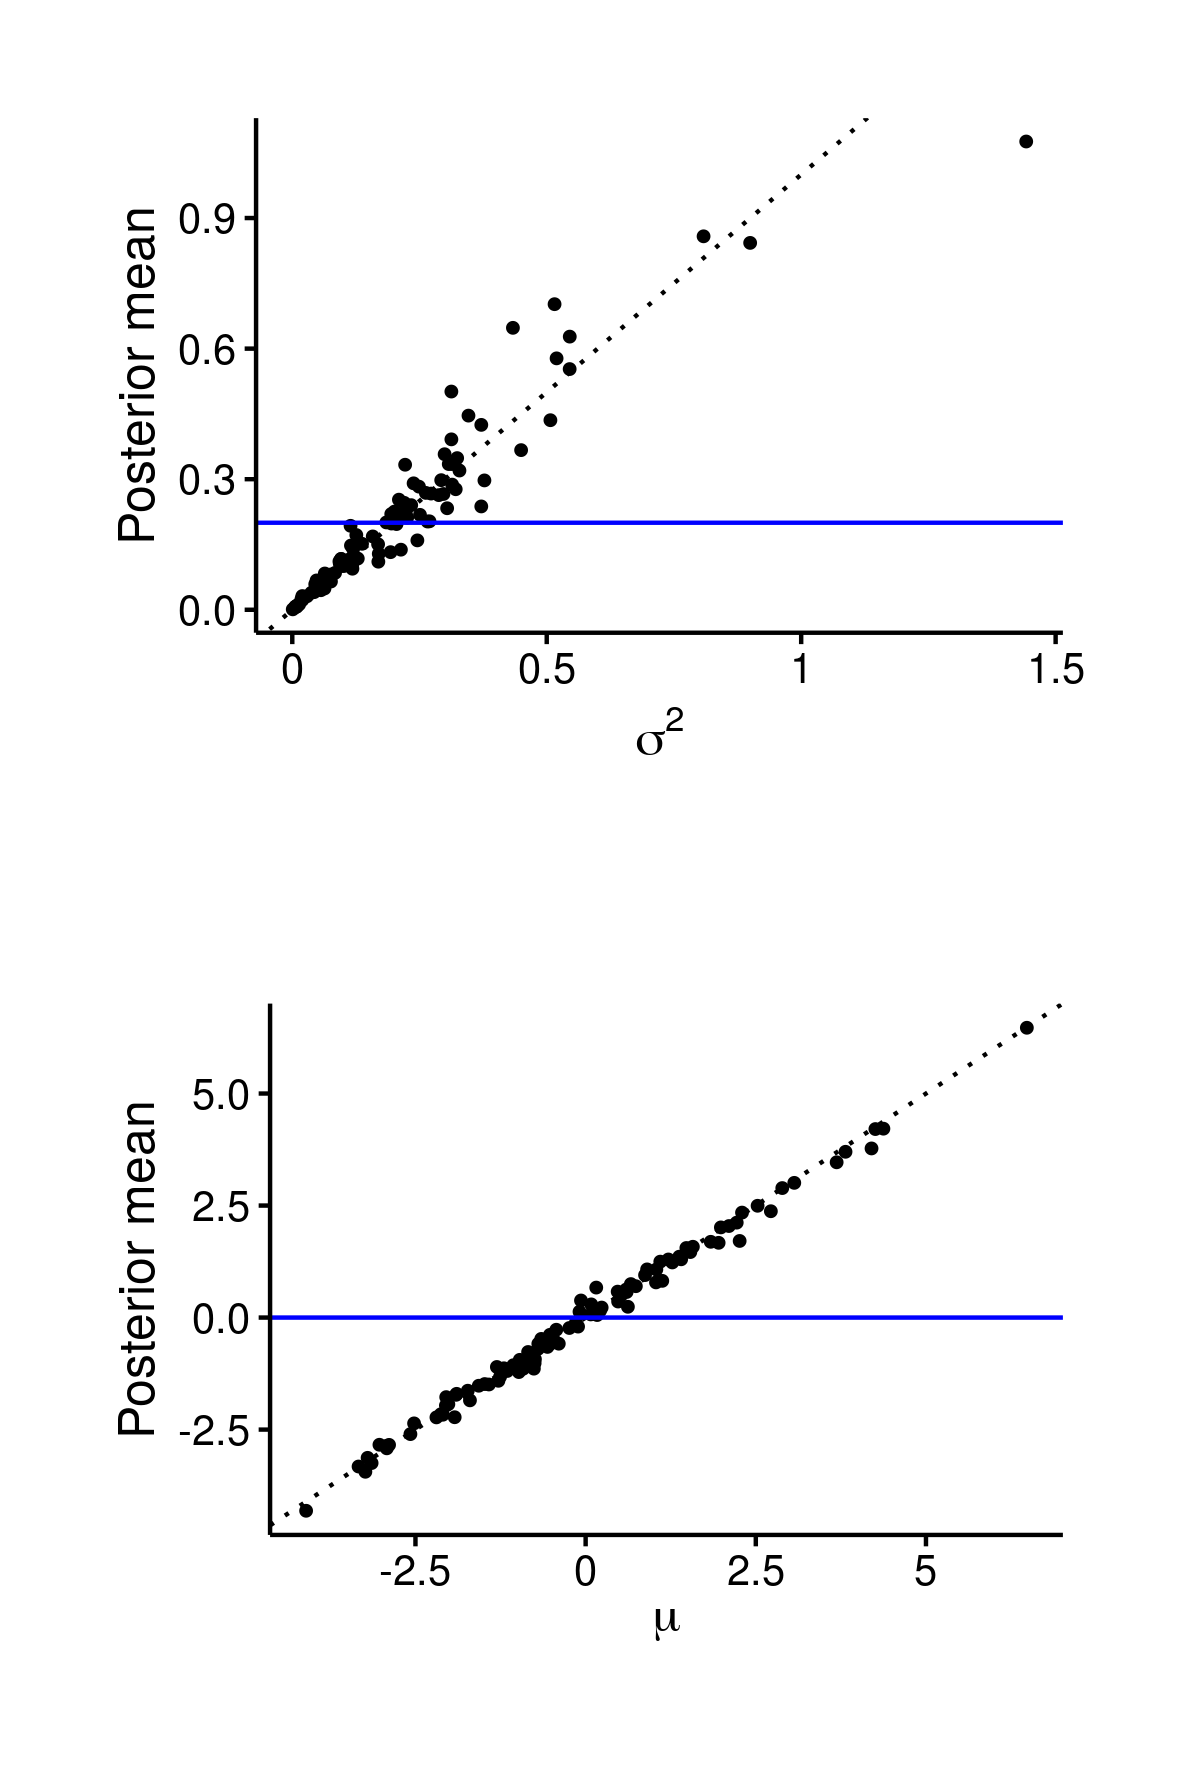
\includegraphics[width=8cm]{../BMMVN_nonultra_graphs.png}
  \end{minipage}
  % \caption{The caption for both}
  % \label{mylabel:1}
\end{figure}

\begin{center}
\begin{tabular}{c | c}
    Parameter & Coverage (\%) \\\hline
    $\mu$ & 97\\
    $\sigma^2$ & 90
\end{tabular}
\end{center}

\end{document}
